\begin{figure*}[!t]
\centering
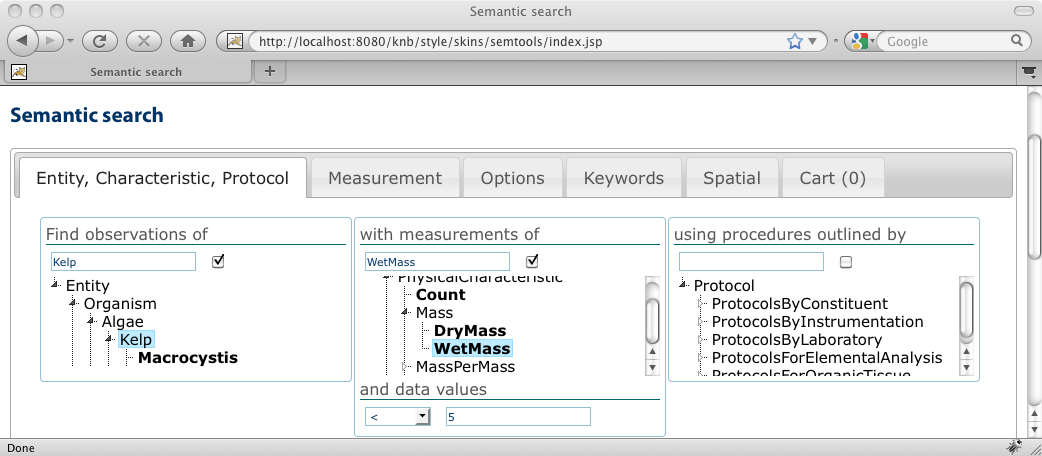
\includegraphics[width=1.0\textwidth]{images/metacat-query.png}
\caption{Semantic data query web interface. Data packages containing observations of Kelp Wet Mass less than or equal to 5 [grams] are returned. Additional search options and compound query criteria can be specified within the other tabs. Matches can be saved in the data cart for later exploration.}
\label{fig:metacat-query}
\end{figure*}


\section{Discovery and Integration}
\label{sec:application}

In this section we describe the new data discovery and integration
applications we have built using the components described above as
part of the Semtools project.

\mypara{Concept query.} The semantic query interface (see
\figref{fig:metacat-query}) is implemented as a Web application over
Metacat that primarily supports locating data sets by how well their
observational models match the given criteria. The interface provides
\emph{structured} as opposed to \emph{unstructured}, i.e.,
keyword-based queries. In particular, query criteria given by users
largely mirror the structure of a semantic annotation in that
combinations of Entity, Characteristic, and Protocol are specified and
optionally compounded when increased precision is sought.

As discussed above, by leveraging the relationships defined and
inferred from the ontology we are able to increase recall beyond what
is possible for simple keyword-based searches
\cite{berkley09:_improv_data_discov_for_metad}. Broad queries return
direct matches as well as subclass matches. The queries can be quickly
refined when using the Web application by allowing rapid exploration
of the data repository without having to define complete observational
queries \emph{de novo}. The interface allows users to specify
individual classes of a measurement as well as pre-configured
measurement types (representing standard data set attribute types) as
defined in OBOE compatible ontologies to enable a single concept to
proxy its constituent parts, namely the characteristics of particular
entities that can be measured with a set of protocols and
standards. This short-hand query generation can save users time in
specifying their queries, and highlights a compelling reason for using
OBOE extension ontologies. Measurement templates can also be leveraged when creating or
editing semantic annotations in the Morpho interface.

Using compound semantic query criteria applies a finer-grained filter
on the data sets that are returned. Results can be restricted to only
those data sets that include measurements for a set of specific
characteristics of a particular observational entity. Furthermore, a
query can specify that those measurements come from precisely the
\emph{same instance of that entity}; a feature that fully exercises
the comprehensive observational structure expressed in the annotation
and enables higher query precision as described above.

\mypara{Data-level query.} For even more precise recall, the OBOE
model can be (partially) materialized (see above) during the query
stage after which a data range filter can be applied. Different
techniques are available for merging the annotation with the data that
it describes, but for performance reasons a hybrid approach has been
adopted in which preliminary search results from a structured query
are collated and only that subset is materialized. Because our corpus
is described using EML in conjunction with the annotation syntax, the
Data Manager Library \cite{leinfelder10:_metad_driven_approac_to_loadin} is used to load the described
raw data (into a relational database) while the annotation informs the
correct use of the Data Manager query and filtering features. For any
measurements that match the concept query criteria, we verify that
those measurements (e.g., attributes) contain data values within the
range specified in the initial semantic data query and return the data
packages that contain them (see \figref{fig:metacat-query}). 

\mypara{Data integration.} The materialization routine used for
semantic data queries laid the groundwork for enabling data
integration. In addition to inspecting the data for values within a
range and returning the data sets that contain a match, the data
integration feature of the Semtools Web application goes further by
constructing a synthetic data product (table) that represents the
complete results of the query in terms of both the attributes and the
values that are returned. Each original data set may have very
different syntactic structures (e.g. column number, naming, order) but
could share a subset of attributes that are semantically compatible as
defined in accompanying annotations. These compatible, in-common
attributes become the facets and metrics in a synthetic data set; their
values filtered accordingly. \figref{fig:integration} further
illustrates the data integration support provided in the current
implementation of the Web application. Consider two data packages,
denoted by A and B in \figref{fig:integration}.  Annotations (denoted
C and D) are used to determine semantically equivalent data attributes
contained in the data sets (denoted by E and F). The attributes {\tt
  plot} and {\tt site} are considered equivalent measurements of the
characteristic Location; attributes {\tt weight} and {\tt wt} both map
to the same characteristic Mass. The Semantic Mediation API parses
each annotation and then computes an equivalence mapping among
attributes based on their corresponding annotations. The Data Manager
Library is then used to load the data sets and then query each data
set to produce and merge the final, synthetic result data set. 

While this approach provides a preliminary form of data-level
integration, we are currently developing additional algorithms for
determining compatibility of annotated measurements (e.g., to include
unit information such as that gram and ounce are both mass units) and
for converting measurement values using ontologically-defined unit
conversions (e.g., 1000 milligrams in a gram), which will further
support automated data integration through the Web application.


\begin{figure}
\centering
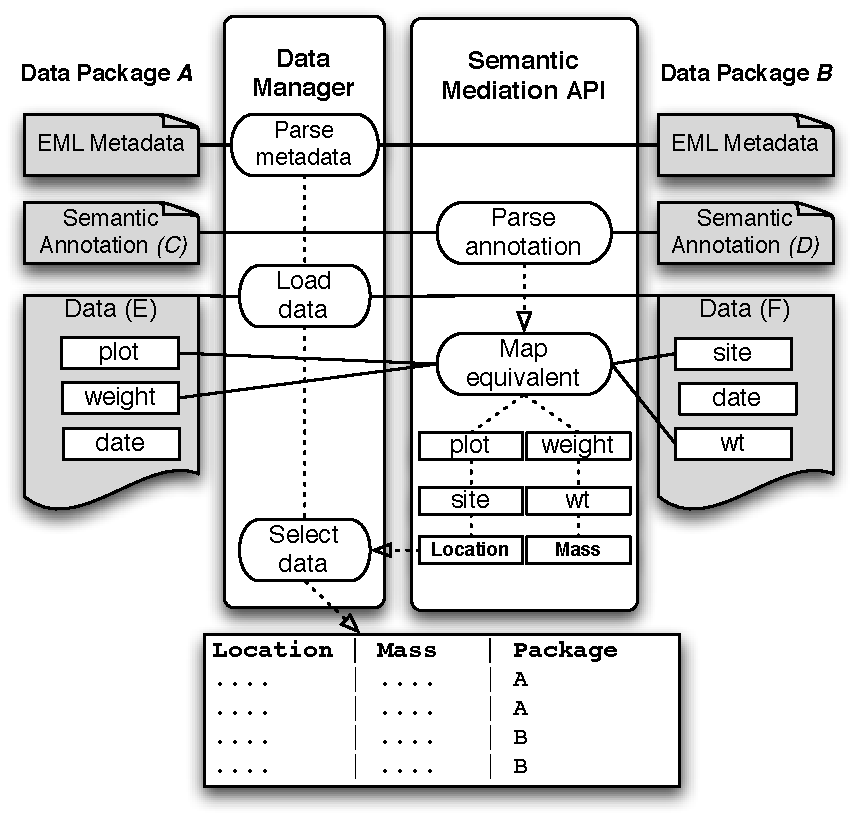
\includegraphics[width=0.45\textwidth]{images/integration.pdf}
\caption{Data integration query across multiple data packages (A, B).
  Annotations (C, D) are used to determine semantically equivalent
  data attributes contained in the data objects (E, F). Attributes
  {\tt plot} and {\tt site} are considered equivalent measurements of the
  characteristic Location; attributes {\tt weight} and {\tt wt} both map to
  the same characteristic Mass. The Semantic Mediation API utilizes
  the Data Manager Library to load and query the source data informed
  by semantic similarities between the structurally disparate data
  attributes.}
\label{fig:integration}
\end{figure}

%%% Local Variables: 
%%% mode: latex
%%% TeX-master: "main"
%%% End: 
